\subsection{Modèle LNAS}
Nous décrivons ici le modèle LNAS (Long Normal Allocation and Senescence) appliqué au blé. C’est un modèle innovant et suffisamment simple pour illustrer tous les enjeux de la thèse. Il est plutôt robuste étant donné sa simplicité, et le faible nombre de données et paramètres requis le rend pratique à l’utilisation. Il traite la production de biomasse au niveau compartemental et peut être considéré comme une simplification du modèle Greenlab qui décrit les même processus au niveau des organes.
C’est un modèle Markovien en temps discret.

\begin{figure}[h]
	\begin{center}
	
	
  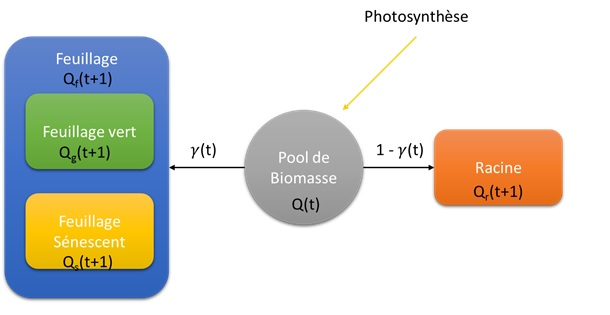
\includegraphics[scale=1.0]{./img/sBeetRoot.jpg}
  \caption{Schéma du modèle LNAS appliqué à la betterave}
  \label{fig:sBeetRoot}
  
  \end{center}
\end{figure}

Le modèle décrit par des fonctions d'allocation comment la biomasse produite quotidiennement est allouée aux différents organes, avec 
\[ o = \{\mathrm{g:grain, s:tige, r:racines, g:feuiles vertes}\} \]

\[ {Q_o^{(n+1)}} = (1-\beta_o^{(n)}-\gamma_o^{(n)} )(Q_o)^{(n)} +\alpha_o^{(n)}q^{(n)} \]

Pour les feuilles jaunes la fonction est différente car elles sont issues de la sénescence des feuilles vertes Q, la production de biomasse. 
Dans ce cas, 
\[ {Q_y^{(n+1)}}=(1-\gamma_y^{(n)})Q_y^{(n)}+Y_l^{(n)}Q_l^{(n)} \]

Les différentes fonctions de circulations dépendent du temps thermique qui peut s'écrire :

\[ {\tau}^{(n+1)}=\tau^{(n)}+\max[0,\underline{T-^{(n)}}-Tc] \]

En supposant que la répartition de biomasse ne commence qu'après un temps caractéristique $\tau_g$ nous pouvons paramétrer la fonction d'allocation $\alpha$ avec la loi log-normale:
\[ {\alpha_g^{(n)}}=F_{\log N(\mu_s,\sigma_g)}(\tau^{(n)}-\tau_g)=\frac{1}{2} (1+erf[\frac{1}{\sigma_g \sqrt{2}}\log (\frac{\tau^{(n)}-\tau_g}{t_{1/2}-\tau_g})]) \]

Les autres fonctions d'allocations peuvent en première approximation être définies comme complémentaires de $\alpha_g$. Le stress hydrique et thermique non détaillé dans ce premier rapport affine notamment la répartition entre racines, tiges et feuilles en plus d'être un possible facteur limitant dans la production de biomasse.

De même pour les fonction de remobilisation $\beta $ et de sénescence $\gamma$, on a
\[ {\beta_o}=\eta_o F_{\log N(\mu_l, \sigma_l)}(\tau-\tau_l) \]
\[ {\gamma_l}=(1-\eta_l)F_{\log N(\mu_l, \sigma_l)}(\tau-\tau_l) \]
\[ {\gamma_y}=F_{\log N(\mu_y, \sigma_y)}(\tau-\tau_y) \]

Le pool de biomasse est la somme de biomasse produit par photosynthèse et de biomasse remobilisée.
\begin{figure}[h]
  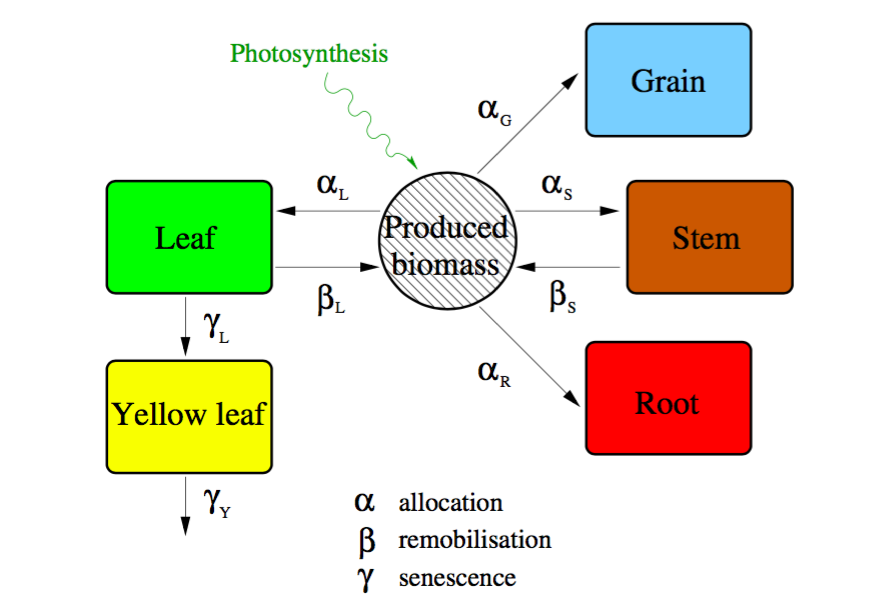
\includegraphics[scale=0.51]{./img/schema-lnas.png}
  \caption{Modélisation de la circulation de biomasse au sein de la plante (modélisée comme un ensemble de compartiments d'organes différents) par des fonctions d'allocation, de remobilisation et de sénescence}
  \label{fig:planning_gant}
\end{figure}

\[ {q^{(n)}}=RUE min[SSI^{(n)}, TSI_\uparrow^{(n)}]PAR^{(n)}(1-e^{-\lambda LAI^{(n)}})+\sum_o \beta_o^{(n)}Q_o^{(n)} \]
\begin{itemize}
\item $\mathrm{Q}(n)$ : Production de biomasse au jour n par unité de surface.
\item $\alpha$  :fonction de répartition
\item $\beta_o$  :fonction de remobilisation
\item $\gamma$ : fonction de sénescence
\item $q^{(n)}$: production de biomasse au jour n 
\item $\mu_g=\log (\tau_{1/2}-\tau_g)$ : espérance de la distribution
\item $\sigma_g$: variance de la distribution
\item $\tau_{1/2}$ : temps thermique où $\alpha_g$ vaut 1/2
\item $erf(x)$: fonction d'erreur
\item $\eta_o$: fraction de biomasse 
\item $RUE$ : efficience de l'utilisation lumineuse
\item $\mathrm{PAR}(t)$ : quantité de radiations photosynthétiquement actives par unité de surface
\item $LAI^{(n)} = S^{(n)}_l/S = \rho_l Q^{(n)}_l $ : Leaf Area Index pour la loi de Beer-Lambert 
\item $\lambda = \sin(\psi)$ avec $\psi$ l'angle moyen des feuilles avec lumière incidente. 
\item $SSI^{(n)}$: indice de stress stomatique (partie hydrique)
\item $TSI^{(n)}$: indice de stress thermique
\end{itemize}
L'équation d'équilibre de l'eau
\[ {R^{(n+1)}}=R^{(n)}+W^{(n)}-Es^{(n)}-Tp{(n)}-d{(n)}\]
L'eau dans la terre dépend de la profondeur z,
\[ {R^{(n)}}=\int_0^{z_M}dz \theta^{(n)}(z) \]
L'évaporation et la transpiration demandées par la plante sont exprimées comme
\[ {Espot^{(n)}}=K_sET0^{(n)}e^{-\lambda LAI^{(n)}}\]
\[ {Tppot^{(n)}}=K_cET0^{(n)}(1-e^{-\lambda LAI^{(n)}})\]

L'eau effectivement transpirée ou évaporée sera le minimum  entre l'évaporation/transpiration requise et l'évaporation/transpiration maximale qui sont calculées selon les propriétés du sol et de la plante (non détaillé dans ce document).

\begin{itemize}
\item $R^{(n)}$: l'eau dans la terre du jour n
\item $W^{(n)}$ : l'eau issue de l'irrigation et de  précipitations au jour n
\item $Es^{(n)}$: l'eau perdue par évaporation depuis la terre
\item $Tp$: transpiration
\item $d$: fonction qui prend en compte la saturation d'eau dans la terre
\end{itemize}
